\documentclass[a4paper, 12pt]{article}
\usepackage{graphicx} % Required for inserting images
\usepackage{fullpage}
\usepackage{amsmath}
\usepackage{xcolor}
\usepackage{float}
\usepackage{geometry}
\usepackage{biblatex}
\geometry{margin=1in}
\usepackage{enumitem}
\usepackage{hyperref}
\usepackage{microtype}

\title{11-24-24 Adding and Subtracting Fractions}
\author{C\&L Math Tutoring}
\date{November 24, 2024}

\begin{document}

\maketitle

\subsection*{Introduction to Fractions}
A \textbf{fraction} represents a part of a whole.
\\\\
The \textbf{numerator} represents the number of parts and the \textbf{denominator} represents the number of parts in the whole.
\\
$$\frac{\text{numerator}}{\text{denominator}}$$

\subsection*{Identifying Fractions}

\begin{figure}[H]
    \centering    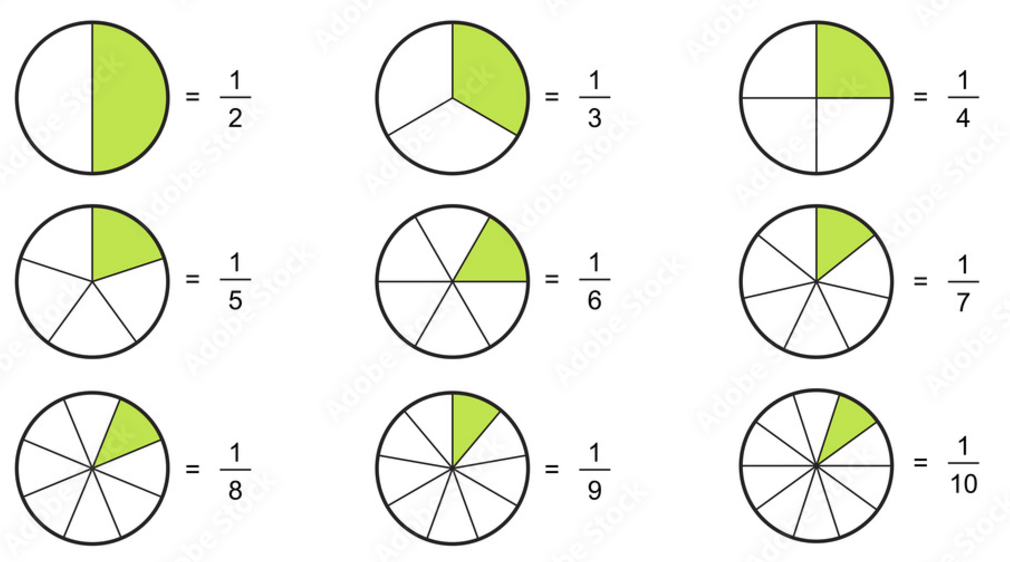
\includegraphics[width=0.7\linewidth]{frac.png}
    \label{fig:1}
\end{figure}

\subsection*{Adding and Subtracting Fractions}
When we add and subtract fractions, we find the \textbf{common denominator} and add the numerators together.
\\\\
Example:
$$\frac{1}{2} + \frac{3}{4} = \: ?$$
\\
\textcolor{blue}{\textbf{Step 1:} Find the LCM} of the two denominators. In this case, the LCM (least common multiple) is 4.
\\\\
\textcolor{blue}{\textbf{Step 2:} Change both denominators} to the LCM by multiplying each fraction by whatever is needed to get to that number.
$$\left(\frac{2}{2}\right) \cdot \left(\frac{1}{2}\right) + \frac{3}{4} = \frac{2}{4} + \frac{3}{4} $$
\\\\
\textcolor{blue}{\textbf{Step 3:} Add the numerators} and put it all over the denominator.
$$= \frac{5}{4} \: \text{or} \: 1\frac{1}{4}$$

\end{document}
